\documentclass[serif,mathserif, 12pt]{beamer}
\usepackage{etex}
\usepackage{amsmath, amsfonts, epsfig, xspace}
\usepackage{algorithm,algorithmic}
\usepackage{pstricks,pst-node}
\usepackage{multimedia}
\usepackage[normal,tight,center]{subfigure}
\setlength{\subfigcapskip}{-.5em}
\usepackage{tkz-euclide}
\usetkzobj{all}
\usepackage{beamerthemesplit}
\usetheme{lankton-keynote}
\usepackage{graphicx,color}
% remove caption of figure
\usepackage[labelformat=empty]{caption}

\usepackage[none]{hyphenat} % hyphenation is ugly in slides
\usepackage{parskip}

\usepackage{relsize} % \smaller to change size

\usepackage{tikz}
\usetikzlibrary{calc}

\usetikzlibrary{arrows}

\newcommand{\TikzDraw}[2][]{
  \begin{tikzpicture}[overlay, remember picture, shift={(current page.center)}, #1]
    #2
  \end{tikzpicture}
}

\newcommand{\gridlines}{
  \TikzDraw{
    \draw[help lines,xstep=.2,ystep=.2,red!20] (current page.south west) grid (current page.north east);
    \draw[help lines,xstep=1,ystep=1,red] (current page.south west) grid (current page.north east);
    \foreach \x in {-15,-14,...,15} {
      \node [anchor=north, red] at (\x,0) {\tiny \x};
      \node [anchor=east,red] at (0,\x) {\tiny \x};
    }
  }
}

\newcommand{\DrawOnImg}[3][]
{
  \begin{tikzpicture}
    \node[anchor=south west,inner sep=0] (image) at (0,0){
      #2
    };
    \begin{scope}[x={(image.south east)},y={(image.north west)}]
      \ifthenelse{\equal{#1}{grid}}
                 {\draw[color=blue, style=dashed] (0,0) grid[xstep=.1, ystep=.1] (1.0001,1.0001);}
                 {}
                 #3
    \end{scope}
  \end{tikzpicture}
}

\usetikzlibrary{matrix}

\newcommand{\BOLD}[1]{\mathbf{#1}}
\newcommand{\BOLDG}[1]{\boldsymbol{#1}}
\newcommand{\PDIF}[2]{\frac{\partial #1}{\partial #2}}
\newcommand{\TODO}[1]{\textcolor{red}{#1}}
\newcommand{\TODOB}[1]{\textcolor{blue}{#1}}
\newcommand{\TODOG}[1]{\textcolor{green!50!black}{#1}}
\newcommand{\argmin}{\operatornamewithlimits{arg\min}}
\DeclareMathOperator{\tr}{tr}
\DeclareMathOperator{\cond}{cond}
\DeclareMathOperator{\ST}{s.t.}
\DeclareMathOperator{\diag}{diag}
\DeclareMathOperator{\Div}{div}

\author{Yin Yang, Weiwei Xu, Xiaohu Guo,\\ Kun Zhou, Baining Guo}

\title[\hspace{2em}\insertframenumber/\inserttotalframenumber]{Boundary-Aware Multidomain Subspace Deformation}
\date{March 20, 2017}

% \institute{Zhejiang University}

\begin{document}

\maketitle

\begin{frame}
  \frametitle{Keywords}
  \begin{itemize}
  \item Subspace method (reduction).
    \pause
  \item Domain decomposition method (DDM)
    \pause
  \item DDM+Subspace (free LMA)
    \pause
    \begin{itemize}
    \item[-] \TODOG{Local deformation, parallelization}
    \item[-] \TODO{Boundary coupling}
      \begin{itemize}
      \item Hard constraint $\rightarrow$ locking
      \item Soft constraint $\rightarrow$ cracks, numerical issue
      \end{itemize}
    \end{itemize}
  \end{itemize}
  \TikzDraw{
    \visible<4-> {
      \node at (4.5, -0.6) {
        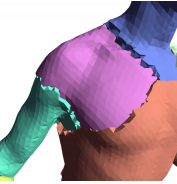
\includegraphics[scale=0.3]{img/cracks}
      };
    }
  }
\end{frame}

\begin{frame}
  \frametitle{Idea}
  \begin{itemize}
  \item Construct boundary-aware subspace bases as compact
    representation of boundary deformation to avoid
    overconstraining problem.
  \end{itemize}
\end{frame}

\begin{frame}
  \frametitle{Background of DDM}
  \begin{itemize}
    \visible<1-> {\item Non-overlapping partition $\Omega = \Omega_1 \cup \dots \cup \Omega_m$
    \begin{equation*}
      R_iA_iR_i^T\Delta \dot q_i = f_i
    \end{equation*}
    }
    \visible<2-> {
  \item Boundary coupling constraint
    \begin{equation*}
      B\Delta \dot q = 0
    \end{equation*}
    }
    \visible<3-> {
  \item Global KKT system
    \begin{equation*}
      \begin{pmatrix}
        H && B^T \\
        B && 0
      \end{pmatrix}
      \begin{pmatrix}
        \Delta \dot q \\
        \lambda
      \end{pmatrix}
      =
      \begin{pmatrix}
        f \\
        c
      \end{pmatrix}
    \end{equation*}
    }
  \end{itemize}
  \TikzDraw {
    \visible<1-> {
      \draw[thick] (4, 0) circle (1.2cm);
      \draw[thick] (3.5, -0.5) rectangle (4.5, 0.5);
      \draw[thick] (3.5, -0.5) -- (3.15, -0.85);
      \draw[thick] (4.5, 0.5) -- (4.85, 0.85);
      \draw[thick] (3.5, 0.5) -- (3.15, 0.85);
      \draw[thick] (4.5, -0.5) -- (4.85, -0.85);
      \node at (4, -0.03) {$\Omega_i$};
    }
    \visible<2-> {
      \draw[thick, red] (3.5, 0.5) -- (3.5, -0.5);
      \node at (3.1, 0) {$\Omega_j$};
    }
  }
\end{frame}

\begin{frame}
  \frametitle{Background of DDM}
  \begin{itemize}
  \item Matrix structure
    \begin{equation*}
      H =
      \begin{bmatrix}
        R_0A_0R^T_0 && && && \\
        && R_1A_1R^T_1 && && \\
        && && \ddots && \\
        && && && R_mA_mR^T_m
      \end{bmatrix}
    \end{equation*}
  \item Update rule
    \begin{equation*}
      \begin{split}
        & \Delta \dot q_i = R_iA_i^{-1}R_i^T(f_i-B_i^T\lambda) \\
        & W\lambda = \sum_i B_iR_iA_i^{-1}R_i^Tf_i-c
      \end{split}
    \end{equation*}
  \end{itemize}
\end{frame}

\begin{frame}
  \frametitle{Outline}
  \begin{itemize}
  \item Construct boundary-aware subspace bases.
    \begin{itemize}
    \item[-] First boundary modes.
    \item[-] Then internal modes.
    \end{itemize}
  \item Apply them to DDM framework with linear elasticity.
  \end{itemize}
\end{frame}

\begin{frame}
  \frametitle{Notions}
  \begin{itemize}
  \item Internal DOF set $\mathcal{I}$
  \item Interface (Boundary) DOF set $\mathcal{B}$
  \item $\mathcal{B} = \mathcal{B}_1\cup\mathcal{B}_2\cup \dots \cup \mathcal{B}_k$
  \item $\Phi = \begin{bmatrix}
    \Phi_\mathcal{I} \\
    \Phi_\mathcal{B}
  \end{bmatrix}$
  \end{itemize}
  \TikzDraw {
    \node at (4, 0) {
      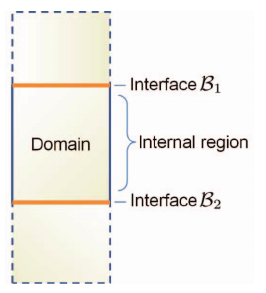
\includegraphics[width=0.35\textwidth]{img/interface}
    };
  }
\end{frame}

\begin{frame}
  \frametitle{Static analysis}
  \begin{itemize}
    \visible<1-> {
  \item Static equilibrium under some boundary conditions
    \begin{equation*}
      \begin{bmatrix}
        K_{\mathcal{II}} && K_{\mathcal{IB}_1} && \dots && K_{\mathcal{IB}_k} \\
        K_{\mathcal{B}_1\mathcal{I}} && K_{\mathcal{B}_1\mathcal{B}_1} && \dots && K_{\mathcal{B}_1\mathcal{B}_k} \\
        & &  & &\vdots & \\
        K_{\mathcal{B}_k\mathcal{I}} && K_{\mathcal{B}_k\mathcal{B}_1} && \dots && K_{\mathcal{B}_k\mathcal{B}_k} \\
      \end{bmatrix}
      \begin{bmatrix}
        \Phi_{\mathcal{I}} \\
        \Phi_{\mathcal{B}}
      \end{bmatrix}
      =
      \begin{bmatrix}
        0 \\
        F_{\mathcal{B}}
      \end{bmatrix}
    \end{equation*}
    }
    \visible<2-> {
  \item Boundary motion
    \begin{equation*}
      \Phi_{\mathcal{B}} =
      \begin{bmatrix}
        \Phi_{\mathcal{B}_1} && && && \\
        && \Phi_{\mathcal{B}_2}  && && \\
        &&  && \ddots && \\
        &&  &&   && \Phi_{\mathcal{B}_k}  \\
      \end{bmatrix}
    \end{equation*}
    } 
  \item \visible<4-> {\TODO{How to characterize boundary deformation?}}
  \end{itemize}
  \TikzDraw {
    \visible<3-> {
      \draw[blue] (-4.6, -2.6) rectangle (-3.6, -1.4);
      \draw[red, thick] (-1.4, -3) rectangle (-0.7, -0.7);
      \draw[red, thick] (-4.6, -1.4) -- (-3.6, -1.4);
      \node at (-4.1, -1.4) {$\mathcal{B}_1$};
    }
  }
  %\gridlines
\end{frame}

\begin{frame}
  \frametitle{Rigid boundary mode $\Phi^R$}
  \begin{itemize}
  \item For $\forall p\in \mathcal{B}_i$ with $c_i$ being center of $\mathcal{B}_i$
    \begin{equation*}
      \Phi^R_p = [x|y|z|(p-c_i)\times x | (p-c_i)\times y | (p-c_i) \times z]
    \end{equation*}
  \item Solve equilibrium
    \begin{equation*}
      \Phi^R =
      \begin{bmatrix}
        \Phi^R_{\mathcal{I}} \\
        \Phi^R_{\mathcal{B}}
      \end{bmatrix}
    \end{equation*}
  \end{itemize}
\end{frame}

\begin{frame}
  \frametitle{Soft boundary mode $\Phi^S$}
  \begin{itemize}
  \item Manifold harmonic bases
    \begin{equation*}
      LH = \Lambda M H
    \end{equation*}
  \item Span in $x, y, z$ directions
    \begin{equation*}
      \Phi_{\mathcal{B}_i}^S = H \otimes Id
    \end{equation*}
  \item Solve equilibrium
    \begin{equation*}
    \Phi^S =
    \begin{bmatrix}
      \Phi_{\mathcal{I}}^S \\
      \Phi_{\mathcal{B}}^S
    \end{bmatrix}
    \end{equation*}
  \end{itemize}
  \TikzDraw {
    \node at (4, 1) {
      \includegraphics[width=0.3\textwidth]{img/dih.pdf}
    };
    \node at (3.8, 1.8) {
      \TODOB{$i$}
    };
    \node at (4, 0.15) {
      \TODOB{$j$}
    };
    \node at (2.8, 0.4) {\TODOB{$\alpha_{i, j}$}};
    \node at (5.6, 0.8) {\TODOB{$\beta_{i, j}$}};
    \node at (0, 1.2) {
      \TODO{$n_{\mathcal{B}_i}\times n_{\mathcal{B}_i}$}
    };
  }
\end{frame}

\begin{frame}
  \frametitle{Rigid vs Soft}
  \begin{itemize}
  \item Rigid versus soft interface
    \begin{figure}
      \centering
      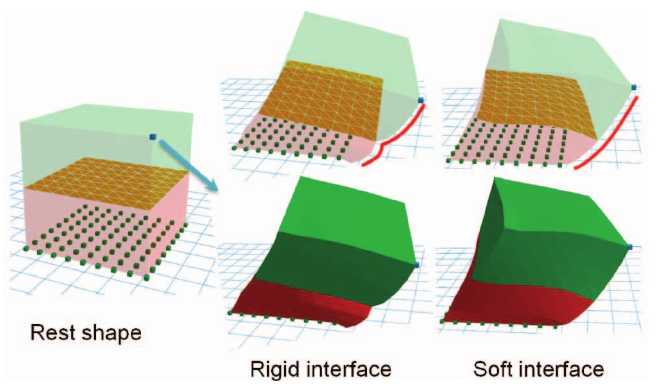
\includegraphics[width=0.8\textwidth]{img/soft_rigid_mode}
    \end{figure}
  \end{itemize}
\end{frame}

\begin{frame}
  \frametitle{Normal internal mode}
  \begin{itemize}
  \item Fix boundary
    \begin{equation*}
      \begin{cases}
        (K_{\mathcal{II}}-\Lambda M_{\mathcal{II}})&\Phi_{\mathcal{I}}^N = 0 \\
        &\Phi_{\mathcal{B}} = 0
      \end{cases}
    \end{equation*}
  \end{itemize}
\end{frame}

\begin{frame}
  \frametitle{Inertia internal mode}
  \begin{itemize}
  \item Inertia forces by boundary acceleration
    \begin{equation*}
      \begin{bmatrix}
        K_{\mathcal{II}} && K_{\mathcal{IB}} \\
        K_{\mathcal{BI}} && K_{\mathcal{BB}}
      \end{bmatrix}
      \begin{bmatrix}
        \Phi_{\mathcal{I}(1)}^I \\
        0
      \end{bmatrix}
      =
      M\Phi^R+
      \begin{bmatrix}
        0 \\
        F_\mathcal{B}^I
      \end{bmatrix}
    \end{equation*}
  \item Iterative mode generation
    \begin{equation*}
      \Phi_{(k+1)}^I =
      \begin{bmatrix}
        \Phi^I_{\mathcal{I}(k+1)} \\
        0
      \end{bmatrix}
      =
      \begin{bmatrix}
        K^{-1}_{\mathcal{II}}M_{\mathcal{II}}\Phi^I_{\mathcal{I}(k)} \\
        0
      \end{bmatrix}
    \end{equation*}
  \item Cascade
    \begin{equation*}
      \Phi_{\mathcal{I}}^I =
      \begin{bmatrix}
        A\Phi_\mathcal{I}^R &&  A^2\Phi_\mathcal{I}^R &&  A^3\Phi_\mathcal{I}^R && \dots
      \end{bmatrix}
    \end{equation*}
  \end{itemize}
\end{frame}

\begin{frame}
  \frametitle{Discussion}
  \begin{itemize}
  \item Layered subspace
    \visible<1> {
    \begin{figure}
      \centering
      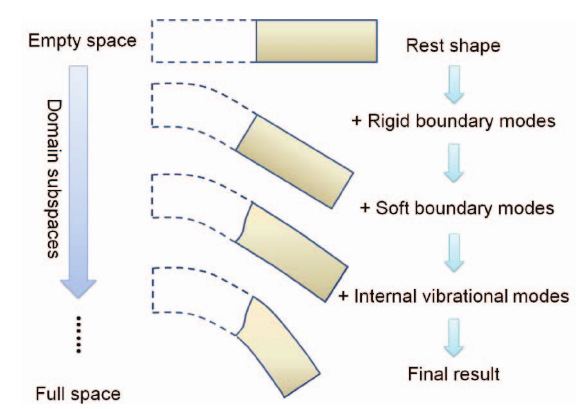
\includegraphics[width=0.75\textwidth]{img/layered_subspace}
    \end{figure}
    }
  \end{itemize}
  \TikzDraw {
    \visible<2-> {
      \node at (0, -0.5) {
        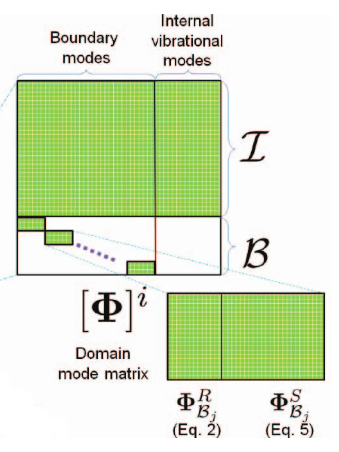
\includegraphics[width=0.4\textwidth]{img/base_patt}
      };
    }
  }
\end{frame}

\begin{frame}
  \frametitle{Discussion}
  \begin{itemize}
  \item Boundary aware versus free LMA
    \begin{figure}
      \centering
      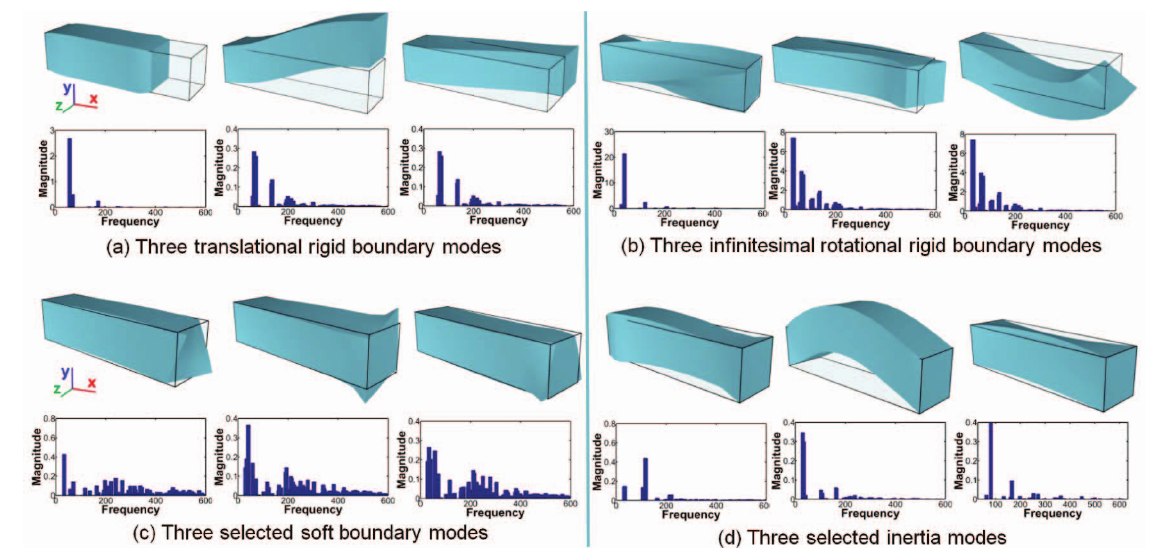
\includegraphics[width=0.9\textwidth]{img/bnd_vs_LMA}
    \end{figure}
  \end{itemize}
\end{frame}

\begin{frame}
  \frametitle{Deformation}
  \begin{itemize}
  \item Equation of motion
    \begin{equation*}
      [M_q]^i[\ddot q]^i+[D_q]^i[\dot q]^i+[K_q]^i[q]^i = [f_q]^i
    \end{equation*}
    \pause
  \item Boundary coupling
    \begin{equation*}
      [\Phi_{\mathcal{B}_i}]^\alpha [q]^\alpha-[\Phi_{\mathcal{B}_i}]^\beta [q]^\beta = 0
    \end{equation*}
    \pause
  \item Large deformation
    \begin{itemize}
    \item[-] modal warping
    \end{itemize}
    \pause
  \item Interaction
    \begin{itemize}
    \item[-] additional PC mode.
    \end{itemize}
  \end{itemize}
  \TikzDraw {
    \visible<4> {
      \node at (2.5, -2.2) {
        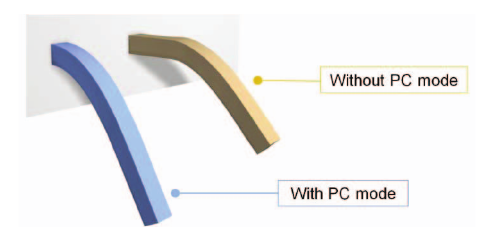
\includegraphics[width=0.45\textwidth]{img/pc_mode}
      };
      \node at (4.5, -1) {
        \TODOB{\small{$\Phi^{PC}=
        \begin{bmatrix}
          -K^{-1}_{\mathcal{II}}K_{\mathcal{IC}} \\
          I_{\mathcal{C}}^{PC} \\
          0
        \end{bmatrix}$}}
      };
    }
  }
\end{frame}

\begin{frame}
  \frametitle{Results}
  \begin{itemize}
  \item Accuracy
    \begin{figure}
      \centering
      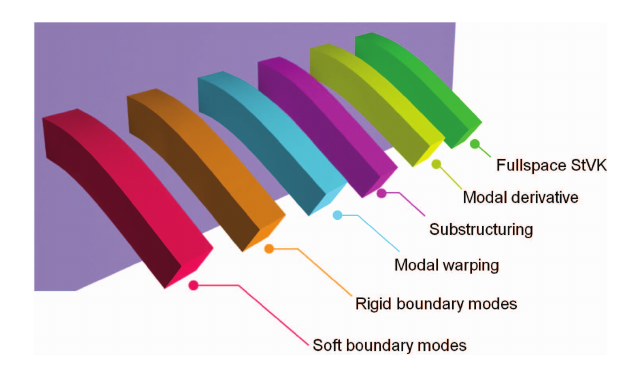
\includegraphics[width=\textwidth]{img/accuracy_comp}
    \end{figure}
  \end{itemize}
  \TikzDraw {
    \definecolor{Mycolor1}{HTML}{C2D812}
    \node at (5.3, -1.3) {\textcolor{Mycolor1}{7.36\%}};
    \definecolor{Mycolor2}{HTML}{AA2597}        
    \node at (4.8, -1.9) {\textcolor{Mycolor2}{13.04\%}};
    \definecolor{Mycolor3}{HTML}{52C1D6}
    \node at (4.4, -2.5) {\textcolor{Mycolor3}{13.21\%}};
    \definecolor{Mycolor4}{HTML}{CD7719}
    \node at (4.0, -3.2) {\textcolor{Mycolor4}{10.35\%}};
    \definecolor{Mycolor5}{HTML}{D4134D}
    \node at (3.6, -3.9) {\textcolor{Mycolor5}{8.45\%}};
  }
\end{frame}

\begin{frame}
  \frametitle{Results}
  \begin{itemize}
  \item Boundary coupling
    \begin{figure}
      \centering
      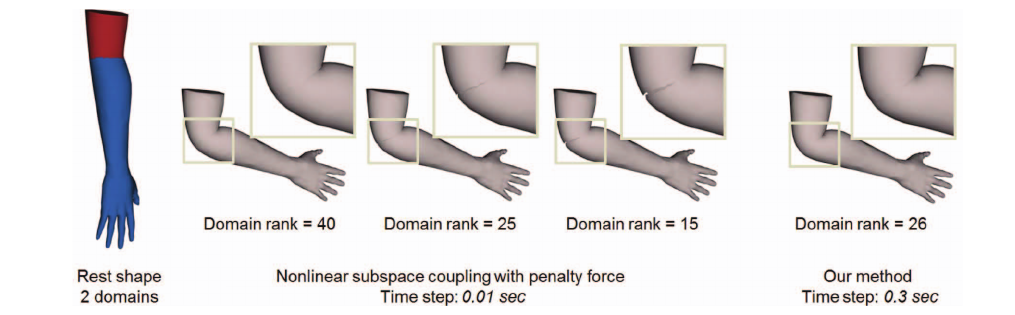
\includegraphics[width=\textwidth]{img/coupling_comp}
    \end{figure}
  \end{itemize}
\end{frame}

\begin{frame}
  \frametitle{Results}
  \begin{itemize}
  \item Large deformation
    \begin{figure}
      \centering
      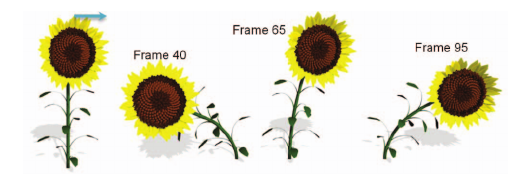
\includegraphics[width=0.8\textwidth]{img/sunflower_large_def}
    \end{figure}
  \end{itemize}
\end{frame}

\begin{frame}
  \frametitle{Results}
  \TikzDraw {
    \node at (-4, 1.5) {
      Performance
    };
    \node at (0, 0) {
      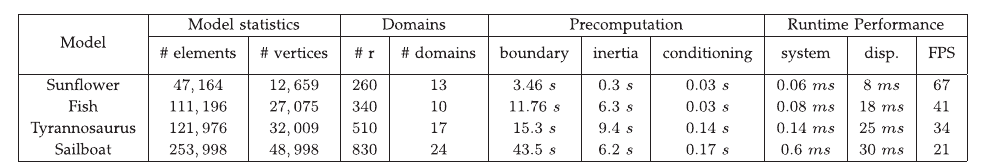
\includegraphics[width=1.1\textwidth]{img/timing}
    };
  }
\end{frame}

\begin{frame} 
  \TikzDraw {
    \node at (0, 0.5) {\Huge{Thanks!}};
  }
  %\gridlines
\end{frame}

\end{document}
